\subsubsection{Energy Data Collection}\label{subsubsec:intro-data-collection}
Energy data collection will be done using the RAPL interface, which is widely accepted as a sufficiently reliable method of
measuring energy[SOURCES].
It provides a simple interface for retrieving energy usage, and breaks down energy usage into multiple domains, which can
be examined separately.
It should be noted that throughout this report we focus on the \textbf{PSys} domain, which contains a slightly more
complete picture of the energy usage of the system that the other domains - this domain is unfortunately not widely
available on all processor models\cite{RAPLDomainInfo}, [TODO: DOUBLE CHECK THIS SOURCE WHEN AAU SITE IS BACK UP] and so the results of this report may not be repeatable on other systems.

The RAPL interface has multiple points of access, which on Linux all depend on the \textit{powercap}
framework\cite{LinuxPowerCap} this section will explore the best approaches to collecting data from RAPL to get the best
test results.
For the purposes of our experiments we will retrieve the energy values in micro-Joules directly from the framework (this
can be done simply by reading the files exposed in the powercap interface).
Our method for retrieving this data is to manually find where each RAPL domain is stored, and retrieving the number that
is stored there - later we can compare these numbers to retrieve a delta of energy usage.
To have a better idea of the energy usage throughout a script's execution, we will retrieve the energy usage at regular
intervals throughout the script's execution, this will also help identify any anomalous behaviour in the energy usage.
The disadvantage of this is similar to the disadvantage of physical energy meters, as there is no way to guarantee that
the beginning of the script is synced with the first energy reading, multiple experiments can mitigate this issue.

The first and easiest way to measure the energy usage of a script is to measure the energy before and after, this
functionality is provided quite simply via the perf tool.
To understand the affect of individual constructs on execution time, there is a need for a more granular measurement of
energy, this can be done one of two ways - either by injecting energy measurements into the scripts themselves, or
by having a separate process measuring the energy level at specified intervals.
The first approach has the advantage of being able to measure the energy usage of the components themselves, while the
second approach is much less invasive and can be applied broadly.
Due to the structured nature of RAPL interface writes, an outside polling approach seems to be more advantageous, as
more granular measurements will not necessarily provide additional data - although this does introduce the possibility
of synchronisation issues between the script and the polling process.

Our first attempt at a polling process for energy usage is with the use of a cron job that runs every second, the job
is simply a bash script that saves data points to a logfile that can then be plotted.

Unfortunately cron does not expose the ability to run a job at a higher frequency than once a minute, so we must
implement a script that executes the polling process in a loop at 1 second intervals.
This has two disadvantages: firstly, if there is any interruption of the script, the polling process will be offset (
if the script is delayed by a second, then there will be a 2-second gap between measurements, and consequently a
duplicate value at the start of the next minute); additionally, as the script executes in non-zero time, every execution
will delay the next poll, this means that the interval does not remain consistent even with perfect execution.
Finally, in the event that the results of this report are to be reproduced, it should be noted that the cron service is
not a guaranteed part of all Linux systems, and may have to be manually installed.

\begin{figure}[H]
    \centering
    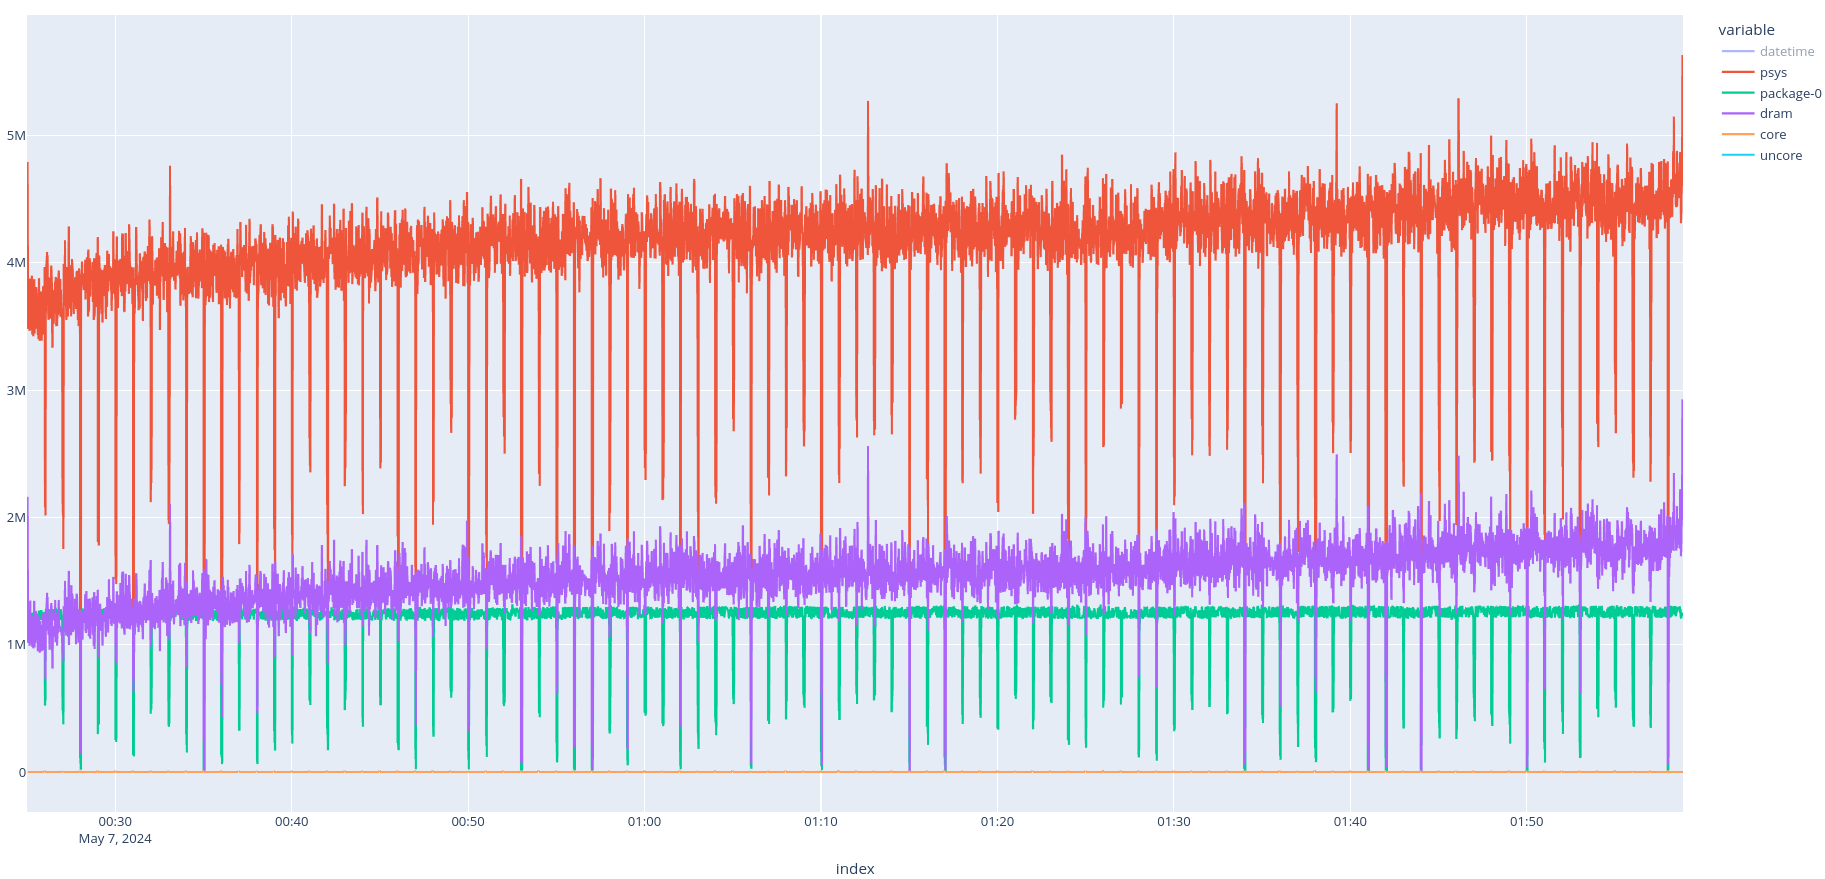
\includegraphics[width=15cm]{figures/introduction/crontab_energy_polling}
    \caption{Using crontab to poll for energy usage every second, the inconsistency of intervals can be seen to cause
    spikes in the data that would have to be normalised for a more accurate representation of the data.}
    \label{fig:crontab_energy_polling}
\end{figure}

The next logical step is to attempt to take advantage of the systemd service manager, which allows creation of custom
daemon services, this includes a timer functionality that allows us to run a polling script every second.
As we can see in fig.\ref{fig:systemd_energy_polling}, the systemd service provides a more consistent interval between
polls, which reduces variance.

\begin{figure}[H]
    \centering
    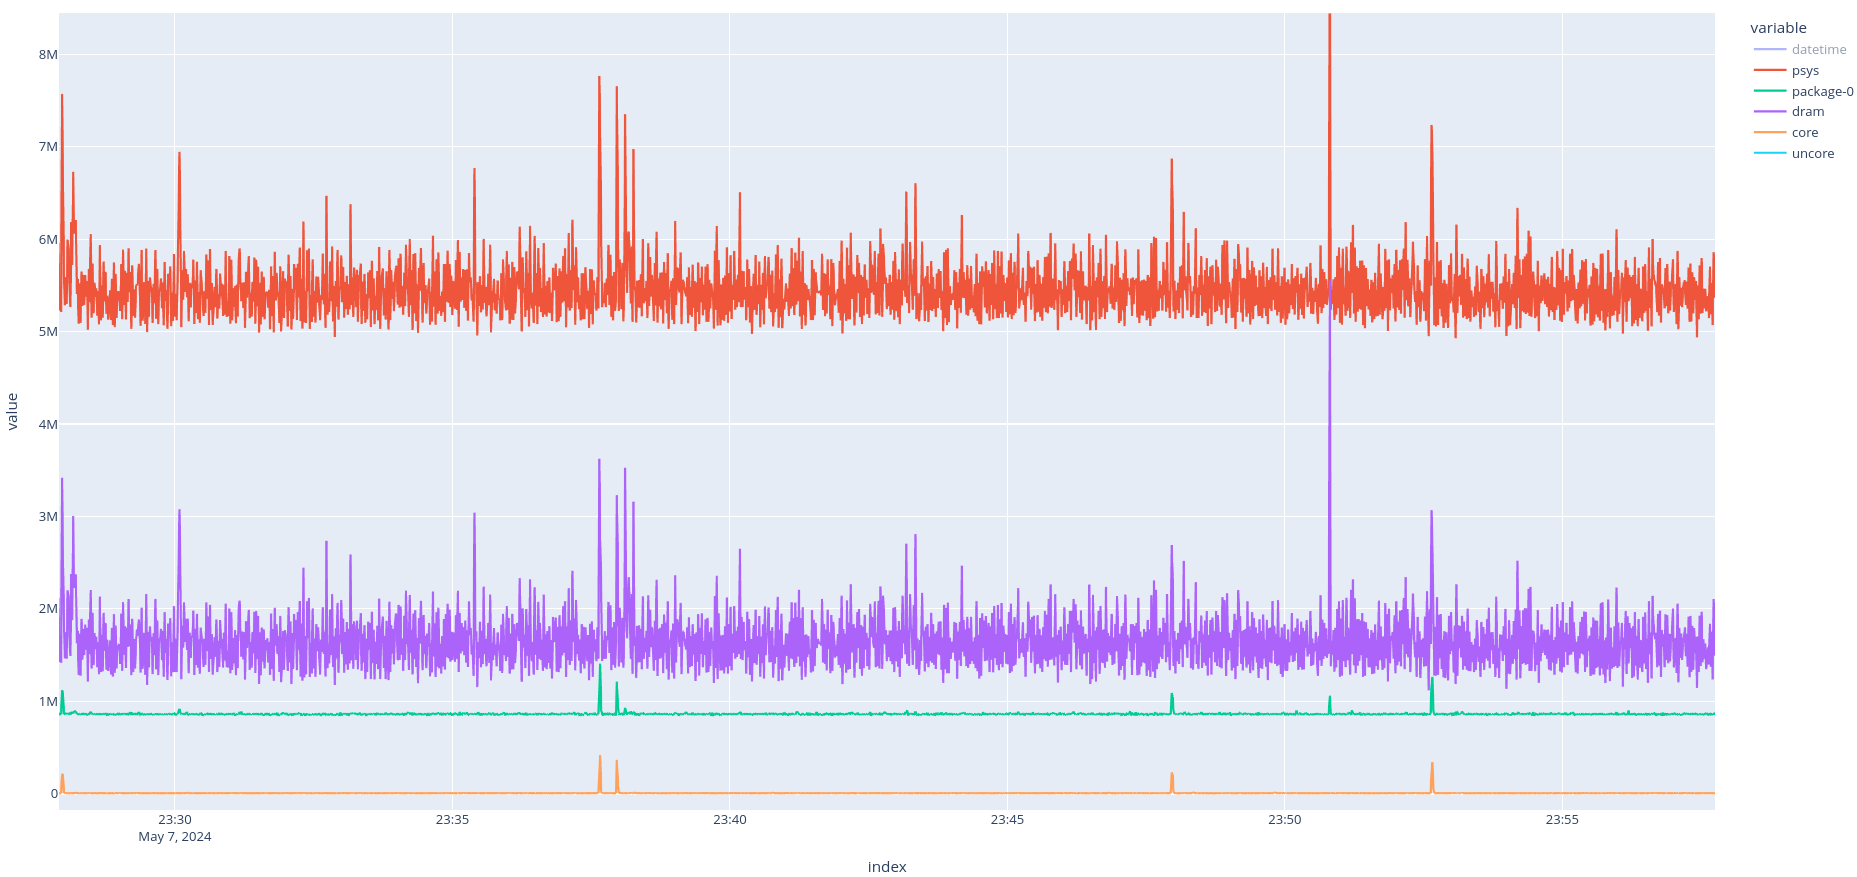
\includegraphics[width=15cm]{figures/introduction/systemd_energy_polling}
    \caption{Using systemd to poll for energy usage every second, the consistency of intervals can be seen to provide a
    more consistent data set, however there is still clear visible variation in the data that may pollute results}
    \label{fig:systemd_energy_polling}
\end{figure}



\subsubsection{Supplementary Data Collection}
In the interest of a full picture, we also retrieve the temperature statistics of the machine, as it may help to
explain anomalous behaviour in the results we find.
This is simply done by parsing the output from the sensors command, which provides the temperature of the CPU cores.
[SOURCE ON SENSORS COMMAND ACCURACY]
Unfortunately the senors command does not provide functionality to request specific data, so some post processing is
required to achieve plottable output - this is done by using the awk command to extract the relevant data, and can be
seen on line 7 in listing~\ref{lst:powerlog-script}.
For plotting, we have chosen to simply average the temperatures of all cores, which may lead to an over-representation
of multithreaded workloads, as the CPU will be hotter when all cores are in use.

For this report we have chosen not to log the workload of the CPU, a technique used by the Scaphandre tool~\cite{ScaphandrePowerConsumption}
This has been done as a time constraint, as analysing the workload of the CPU would require a significant amount of
analysis to determine the effect of each workload on energy usage.


\subsubsection{Polling Frequency}
The first step in data collection is to determine the frequency at which we will poll the system, this is important as
higher poll rates will affect the system more, while providing more accurate data.
Intel claims an update frequency of approximately 1 millisecond\cite{RAPLInterface}, providing an upper limit for viable
frequency, however the value that we choose will likely be lower than this, due to the time required to read from the
RAPL interface.
As it is impossible to guarantee exact intervals (to within microseconds), we will normalize all results to
Joules/second, this will also prevent higher poll frequencies from having lower energy readings, allowing for easeier
comparisons of the true invasiveness of the polling system.

In addition to finding the optimal polling frequency, this section will provide a baseline control dataset that can be
compared against future data.

\textbf{Rate - 1s}
A rate of 1 second produces unremarkable results, as there is a lack of comparison so far.

\begin{figure}[H]
\centering
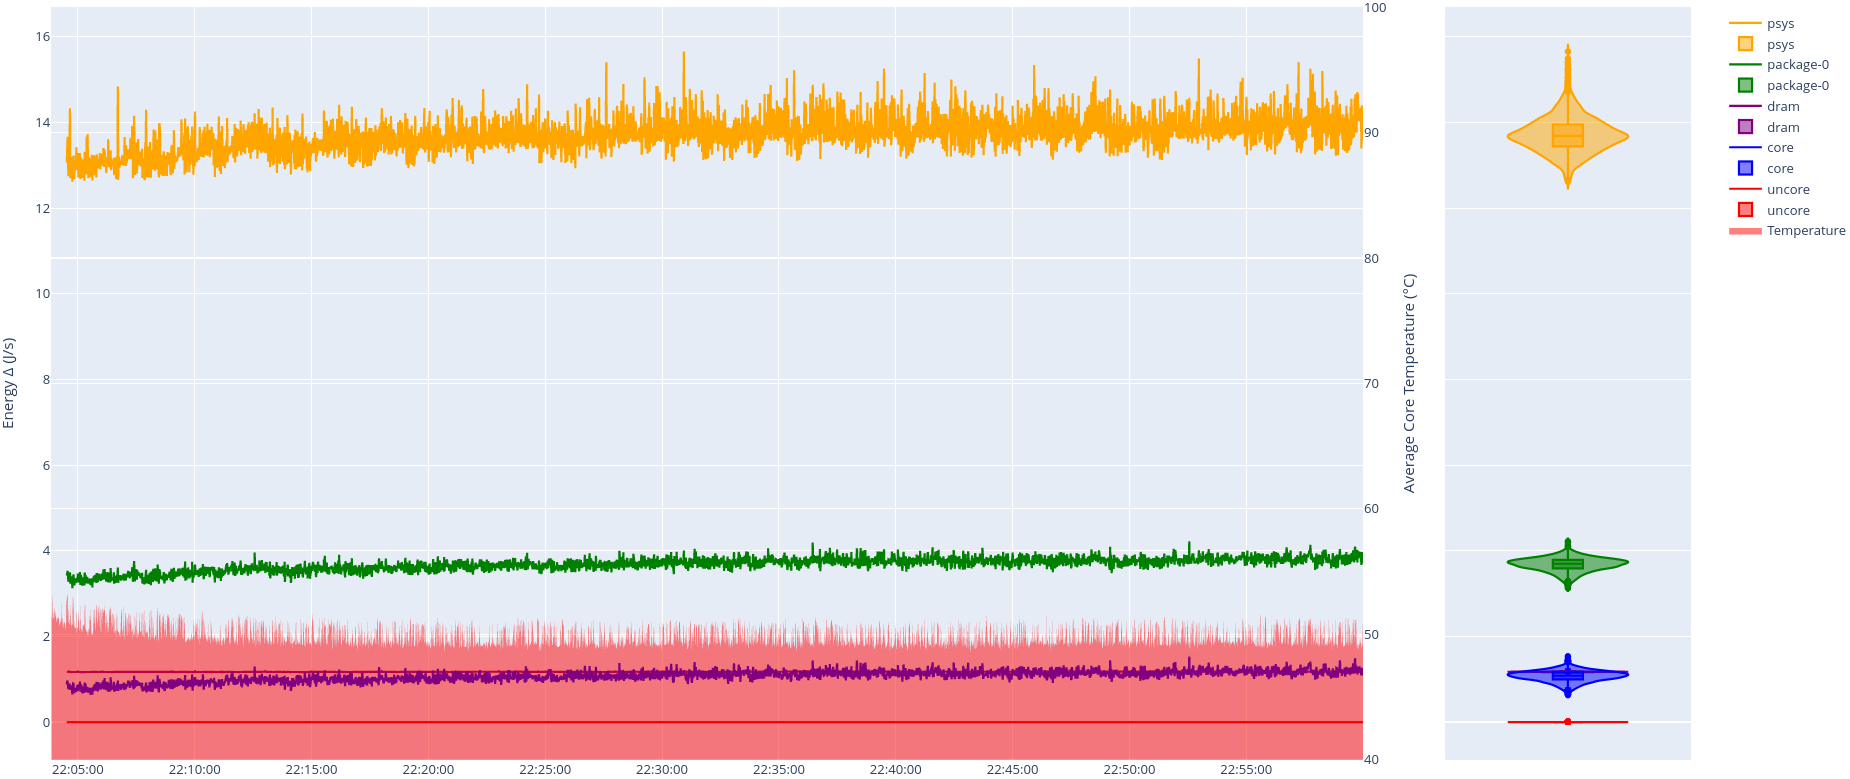
\includegraphics[width=15cm]{figures/implementation/control_sytemd10}
\caption{Polling the powercap interface at a rate of every second for an hour; psys stats are: min - 12.61, max - 15.65, mean - 13.70, std - 0.41}
\label{fig:systemd10ratetest}
\end{figure}

\textbf{Rate - 0.5s}
A rate of 0.5 seconds has a noticeable increase in power usage, however variance is slightly lower, this could either be
due to random chance, or it may indicate that there is a pattern to the volatility of RAPL's power readings, which
suggest the possibility of modeling the baseline pattern of the system to predict future power usage.
This rate also exposes a cyclical pattern to temperature, which may be useful for future analysis.

\begin{figure}[H]
\centering
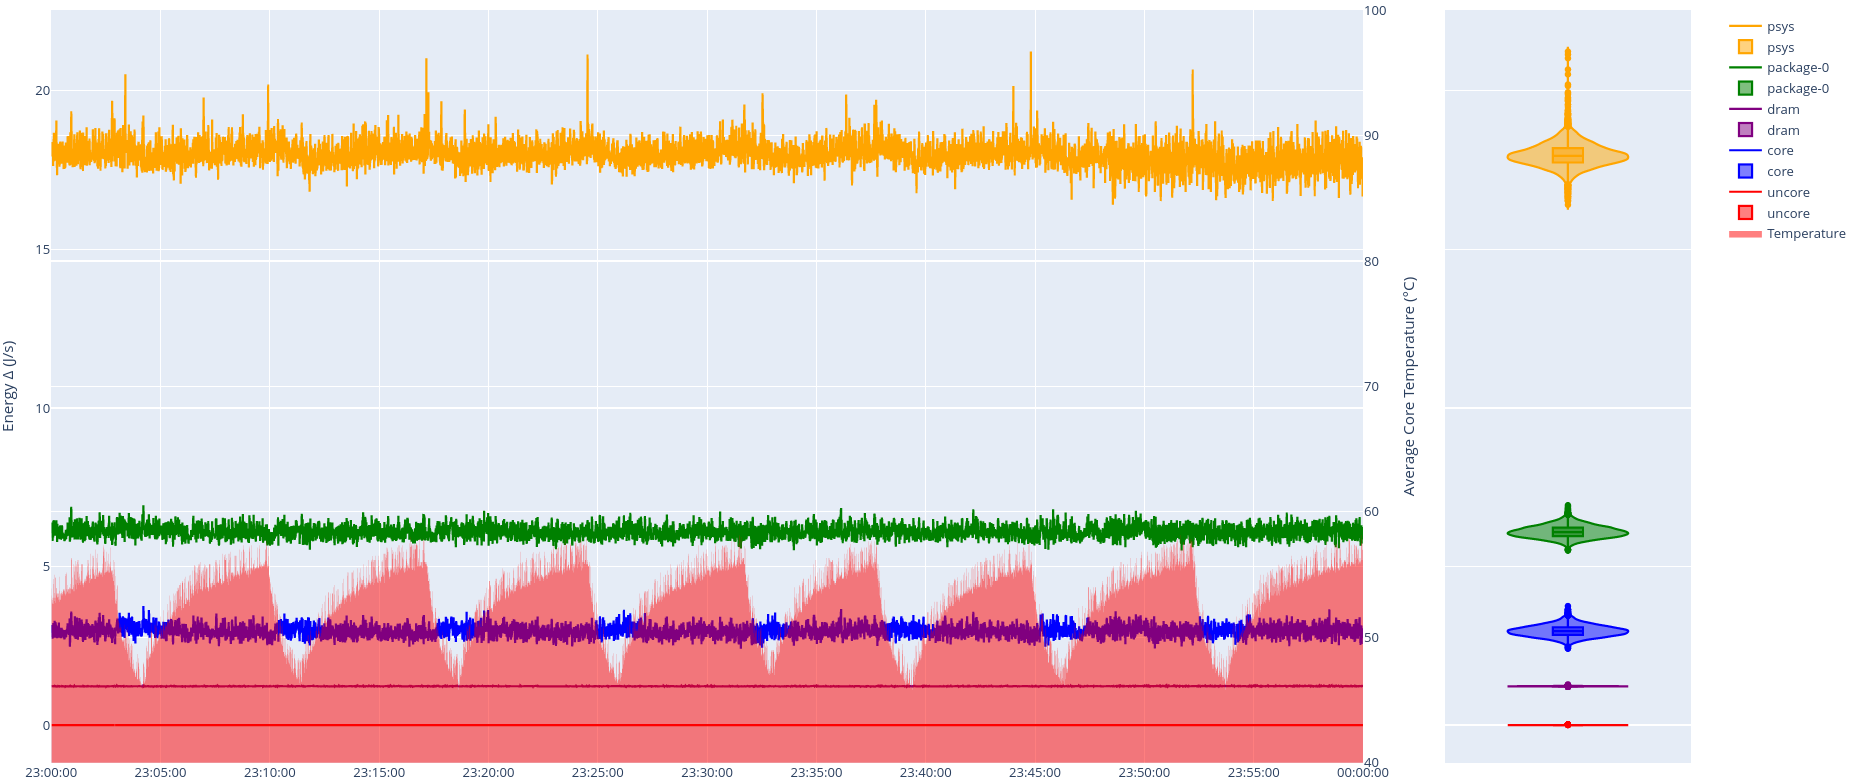
\includegraphics[width=15cm]{figures/implementation/control_systemd05}
\caption{Polling the powercap interface at a rate of every 0.5 seconds for an hour; psys stats are: min - 16.41, max - 21.24, mean - 17.97, std - 0.38}
\label{fig:systemd05ratetest}
\end{figure}

\textbf{Rate - 0.2s}
A rate of 0.2 seconds uses almost double the energy of the 1 second rate, and has much higher variance, making it the
worst choice for a polling rate.

\begin{figure}[H]
\centering
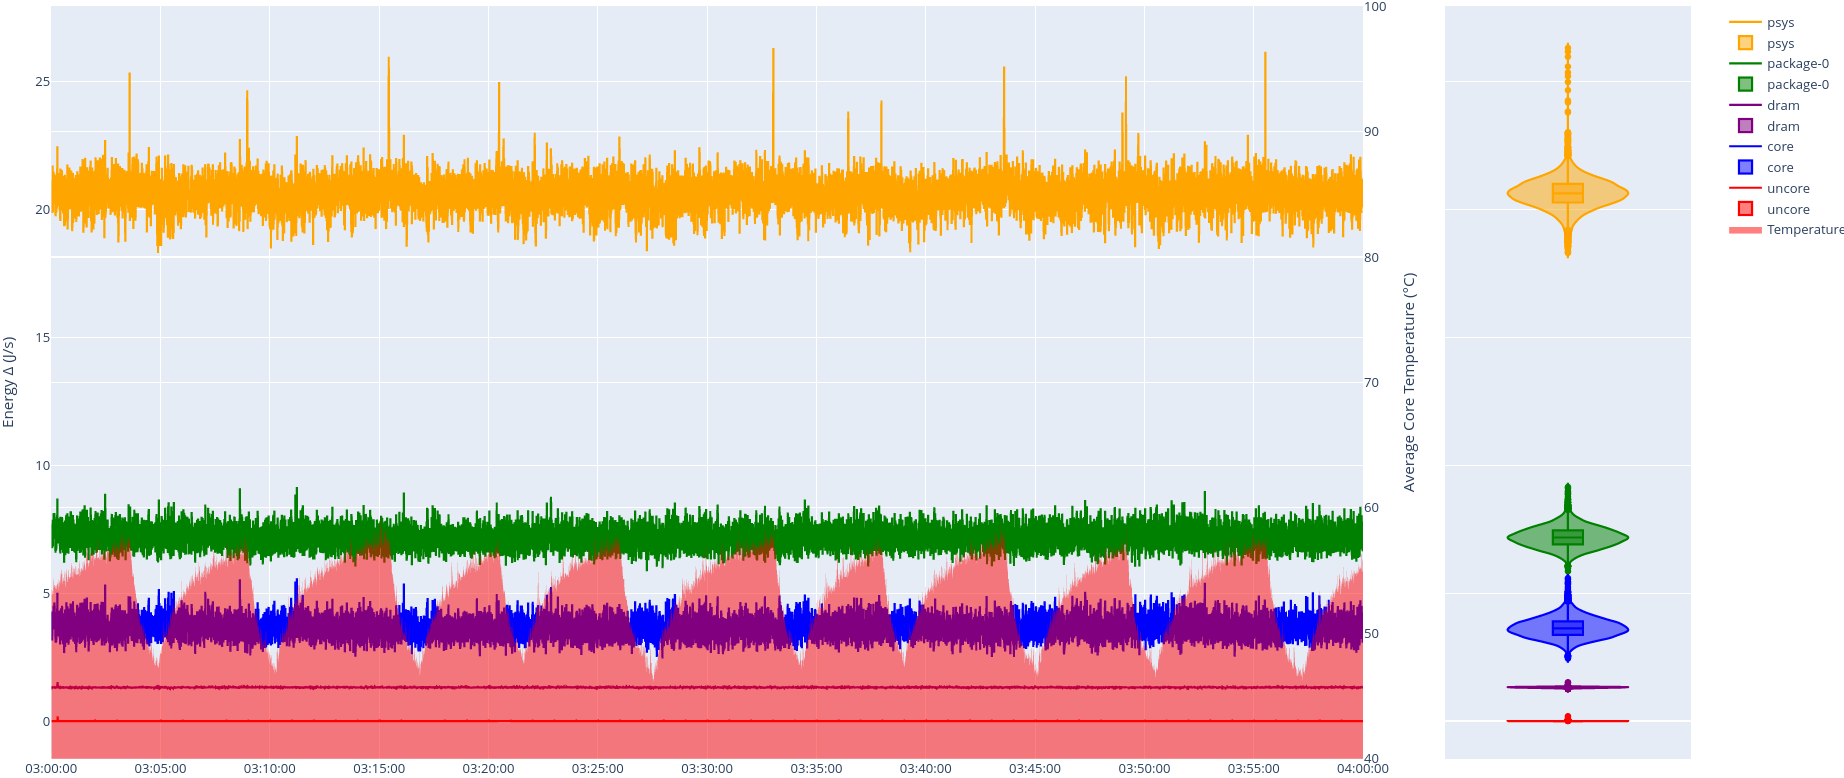
\includegraphics[width=15cm]{figures/implementation/control_systemd02}
\caption{Polling the powercap interface at a rate of every 0.2 seconds for an hour; psys stats are: min - 18.29, max - 26.30, mean - 20.61, std - 0.58}
\label{fig:systemd02ratetest}
\end{figure}


\subsubsection{Conclusion}
Unfortunately increasing the rate past 0.2 seconds appears to crash the systemd process, and has been deemed not viable
for experimentation.
As results are relative, we choose the polling rate of 0.5 seconds, as it provides a good balance between invasiveness
and repeatable patterns - and better models temperature change.
Readers repeating the process may also want to use these results to extrapolate the energy cost of the polling system -
this can be done by taking the difference between the mean of the 0.5s rate and the 1s rate, and then multiplying this
that difference by 2 (note that this is unlikely to be accurate, and is disproved by our results where the difference
between 1 and 0.5 should be smaller than the difference between 0.5 and 0.2).

Lastly, RAPL occasionally resets the powercap interface to zero readings - this interferes with results, as it is no
longer possible to simply compare the power reading before and after results.
Due to the nature of powercap updates, we will never receive a zero value, so the current process is to subtract the
first power usage value from the maximum, and then add the final value - it is important to note that this approach will
not work for experiments that run long enough to have two or more updates.

The resulting collection logic is displayed in listing~\ref{lst:powerlog-script}, this is executed by the systemd service
in listing~\ref{lst:systemd-energy-polling} which is in turn executed by the timer service in listing~\ref{lst:systemd-energy-timer}.

\begin{lstlisting}[caption={power and temperature logging script - variable names have been replaced with hash characters},captionpos=b,label={lst:powerlog-script}]
ENERGYOUT=###############
TEMPOUT=#################
ENERGY_FILE=$(cat ###############)

time=$(date +"%y-%m-%d %T")
energy=$(cat $ENERGY_FILE | sed -z 's/\n/,/g')
temp=$(sensors | awk -F '°' '/^Core/{gsub("[[:space:]]+",""); printf "%s,", $1}')

echo "RUNNING POWERLOG"
printf "$time,$energy\n" >> $ENERGYOUT
printf "$time,$temp\n" >> $TEMPOUT
\end{lstlisting}

\begin{lstlisting}[caption={systemd service},captionpos=b,label={lst:systemd-energy-polling}]
[Unit]
Description=Run profiler every second
StartLimitIntervalSec=60
StartLimitBurst=61

[Service]
ExecStart=/usr/bin/bash #########/powerlog.sh
User=#######

[Install]
WantedBy=multi-user.target
\end{lstlisting}
\begin{lstlisting}[caption={systemd timer},captionpos=b,label={lst:systemd-energy-timer}]
[Timer]
OnUnitActiveSec=1s
AccuracySec=1us
Unit=profiler.service
\end{lstlisting}


